\documentclass{beamer}

\usepackage{graphicx}
\graphicspath{ {./diagrams/} }

\title{Introduction to Git}
\author{Cengiz Kandemir}
\date{\today}

\begin{document}

\frame{\titlepage}

\begin{frame}{Outline}
  \tableofcontents
\end{frame}

\section{Who am I?}
\begin{frame}
  \frametitle{Who am I?}
  \begin{itemize}
  \item[] Currently: Software Engineer @ Sioux, working w/ Philips IGT
  \item[] Before:
    \begin{itemize}
    \item[] Software Engineer @ AirTies
    \item[] Research Assistant @ EMU (co-supervised by Cem Kalyoncu)
    \end{itemize}
  \end{itemize}
\end{frame}

\section{What is Git and why do we need it?}
\begin{frame}
  \frametitle{What is Git?}
  \begin{quote}
    Git is software for \textbf{tracking changes} in any set of files, usually used for \textbf{coordinating work} among programmers collaboratively developing source code during software development. \\ \begin{flushright}Wikipedia\end{flushright}
  \end{quote}
\end{frame}

\begin{frame}
  \frametitle{Why do developers need a version control systems?}
  \begin{itemize}
  \item<1-> Synchronize changes made by two or more developers
  \item<2-> Undo/redo changes conveniently
  \item<3-> Bookmark (aka \textit{tag}) specific points in a repository's history
    \begin{itemize}
    \item<4-> Release/important milestones
    \item<5-> Critical/risky changes
    \end{itemize}
  \item<6-> Improved traceability and visibility
    \begin{itemize}
    \item<7-> Traceability: Bugs can be narrowed down based on the locality of changes
    \item<8-> Visibility: Changes are visible to other stakeholders
      \begin{itemize}
      \item<8-> Improved collaboration
      \end{itemize}
    \end{itemize}
  \item<9-> Improved software quality
    \begin{itemize}
    \item<10-> Testing/Static analysis
    \item<11-> CI/CD pipelines
    \end{itemize}
  \end{itemize}
\end{frame}

\section{Basics of Git}
\begin{frame}
  \frametitle{Git loop}
  \centering
  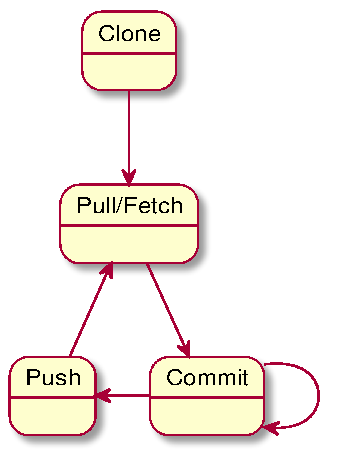
\includegraphics{git_loop}
\end{frame}

\begin{frame}
  \frametitle{git-clone}
  \begin{itemize}
  \item<1-> Clones a git repository (\textit{.git} folder)
  \item<2-> A repository can be located \textit{\textbf{locally}} or \textit{\textbf{remotely}}
  \item<3->[] \textit{git clone} {\textless}\textit{path-to-repo}{\textgreater}
  \end{itemize}
\end{frame}

\begin{frame}
  \frametitle{git-stage \& git-commit}
  \begin{itemize}
  \item<1-> A commit is composed of two steps: staging and committing
  \item<2-> Staging is useful for compartmentalizing changes
  \item<3->[] \textit{git stage} {\textless}\textit{list-of-files-to-be-staged}{\textgreater}
  \item<3->[] \textit{git commit}
  \item<4-> The state of repository after a commit is recorded and can always be returned to
  \item<5-> Committing a set of changes creates a ``bookmark``, identified by a \textit{\textbf{commit hash}}
  \item<6-> Many commands in Git require a commit hash as an input
  \end{itemize}
\end{frame}

\section{Best practices}

\end{document}
%%% Local Variables:
%%% mode: latex
%%% TeX-master: t
%%% End:
